\documentclass[11pt,a4paper]{article}
\usepackage{lac2010}
\usepackage{amssymb,amsmath}
\usepackage{graphicx}
\usepackage{pstricks}

\usepackage{listings}

\sloppy
\newenvironment{contentsmall}{\small}

\title{Emulating a Combo Organ Using Faust}

\author
{Sampo SAVOLAINEN
\\ Foo-plugins
\\ http://foo-plugins.googlecode.com/
\\ sampo.savolainen@gmail.com
}

\begin{document}
\lstset{captionpos=b,tabsize=2,basicstyle=\footnotesize}

\maketitle


\begin{abstract}
\begin{contentsmall}
This paper describes the working principles of a 40 year old transistor organ and how it is emulated with software. The emulation presented in this paper is open source and written in a functional language called Faust. The architecture of the organ proved to be challenging for Faust. The process of writing this emulation highlighted some of Faust's strengths and helped identify ways to improve the language.

\end{contentsmall}
\end{abstract}

\keywords{
\begin{contentsmall}
Faust, synthesis, emulation
\end{contentsmall}
}

\section{Introduction}

Faust\cite{orlarey:09c} stands for Functional AUdio STream and as the name implies it is a functional language designed for audio processing. The Faust compiler is an intermediary compiler, which produces source code for a C++ signal processor class which is integrated into a chosen C++ architecture. This architecture file provides a run-time environment, or wrapper, for the processor. This wrapper can be for example a stand-alone Linux Jack application or an audio processing plug-in.

%% TODO choose license
This paper describes how an emulation of a 1970's combo-organ was written in Faust. The Yamaha YC-20 is a fairly typical organ of its time, a transistor based relatively light instrument meant for musicians on the road. The organ is a divide-down design and its working principles are discussed in detail in section \ref{section:yc-20}. The emulation is released as open source using the GNU General Public License (v3). In the spirit of open source, the working principles and decisions taken during writing the emulation are described in this paper for all to read.

The YC-20 was chosen to be emulated as its architecture is very different from typical software and virtual analog synthesizers. Instead of the complex controllability and routability of typical synthesizers, this organ requires a large number of fixed parallel processes and components. This makes for a good test of Faust's performance and parallelization capabilities. Access to an operational organ was also a factor in the choice, as it makes it possible to match the emulation quality against the original. 

The contents of this paper is organized into four sections. The first section covers how the real organ operates. This is followed by a description of how the organ is emulated. The third section covers the performance aspects of the emulation. The last section offers analysis of Faust's strengths and gives proposals on how to improve the language.

\section{YC-20}
\label{section:yc-20}

This section covers the operations of the organ in detail\cite{yamaha:yc20}. The information in this is section is later referred to and detailed further when discussing the emulated parts. Figure \ref{fig:yc20block} shows a block diagram of the device.

\begin{figure}[tbp]
\centering
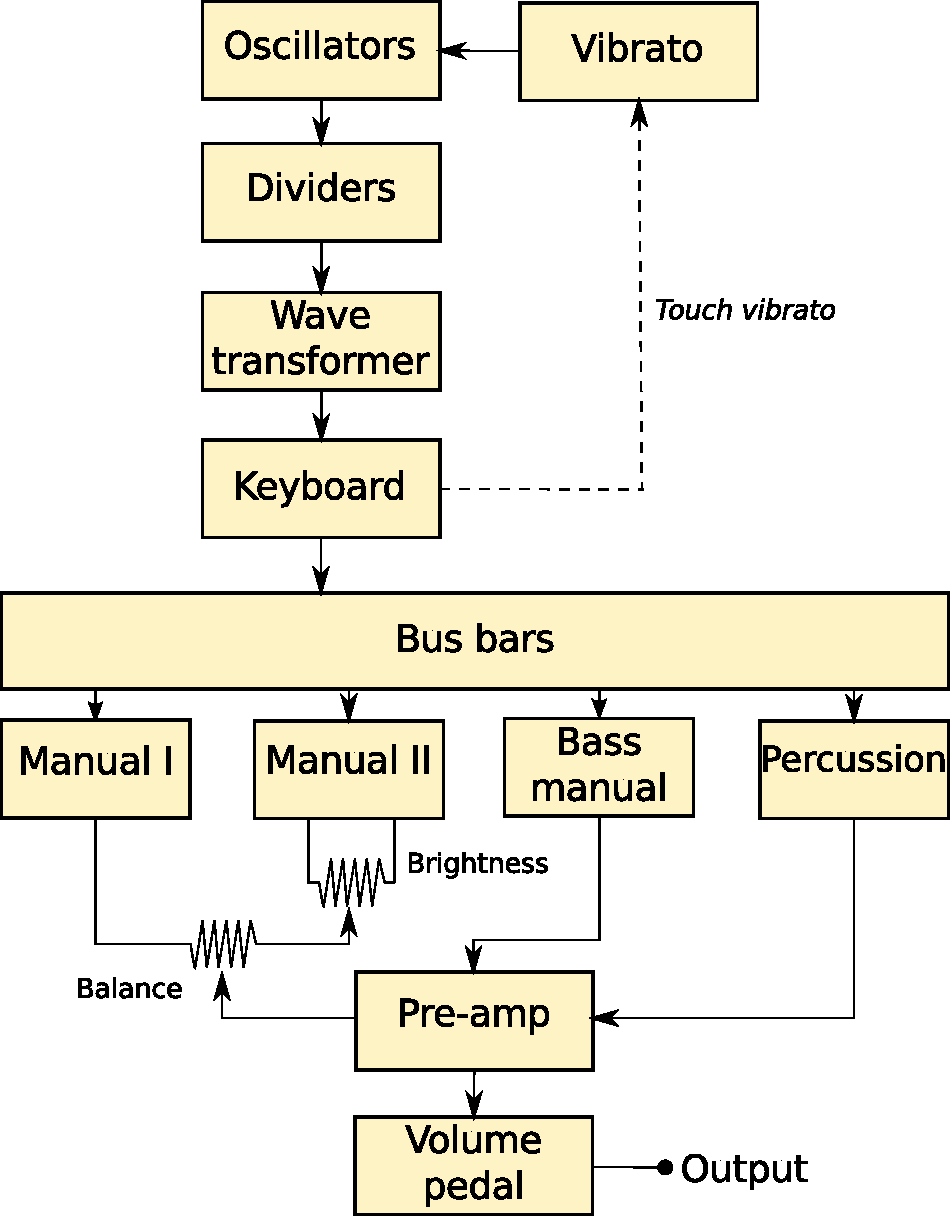
\includegraphics[width=80mm]{yc20-block.pdf}
\caption{Block diagram of the YC-20}
\label{fig:yc20block}
\end{figure}

\subsection{Features}

The organ has one physical manual with 61 keys with a switchable 17 key bass manual and two voice sections. Instead of drawbars like Hammond organs, the voices are controlled by a lever system used in Yamaha organs of the time. As the word drawbar is commonplace when discussing organ voicing, the word is used in place of lever for the voice controls. While the controls are potentiometers, they have notches to help the user achieve repeatable settings. Each drawbar lever in the organ has four positions (end stops and two notches) from off to full volume. 

Section I has drawbars 16', 8', 4', 2-2/3', 2', 1-3/5' and 1' and section II has drawbars 16', 8', 4', 2' and a continuous brightness lever. The sections can be selected or mixed together using a continuous balance lever. Enabling the bass manual switches the lowest 17 keys (white on black) to bass manual with drawbars 16' and 8'. There are also global controls for pitch, volume, bass volume, vibrato depth, vibrato speed and an obscure "touch vibrato" feature. The organ also has a single global percussion drawbar and an integrated volume pedal. Like the drawbars, all vibrato controls have four positions.

% the style of controls? .. probably irrelevant
\subsection{Tone generation}

The synthesizer architecture comprises of 12 oscillators, one per each note in a twelve-tone equal temperament (12-TET) scale. The oscillators produce a sawtooth wave. For each oscillator, there are 7 frequency divider stages so each oscillator produces 8 voices totalling 96 voices. The dividers produce square waves. 

These voices are next fed through a passive filter bank. The divided voices have both a high pass and low pass filters while the oscillator voices are only high pass filtered to remove bias. This totals 180 resistor-capacitor (RC) filter networks. Filtered voices are connected to switches on the actual keys of the keyboard. The keyboard is thus in fact a matrix mixer connecting the voices to bus bars. A key feeds each bus bar with the appropriate voice matching that key and octave, or the matching harmonic voice in case of the 2-2/3' and 1-3/5' bus bars. 

\subsection{Sections}
\label{section:sections}

The drawbar controls are potentiometers which control how much of each bus bar is mixed to each section of the organ. While in section I, drawbars are simply mixed together using resistors, Section II drawbars have more complex filtering. Each section II drawbar is divided into two streams, each filtered separately with RC networks. One stream is low pass filtered while the other is high pass filtered. The low passed and high passed signals are mixed through resistors to combine into bright and dull signals which are then buffered. The brightness potentiometer controls a mix of the two which, after further buffering, is the output of section II. 

The key switches on the lowest 17 keys feed either separate bass bus bars. The bass manual switch controls whether these bus bars are kept separate or mixed with the main bus bars. Thus, with the bass feature disabled, the bass keys work exactly as the rest of the manual. With the switch enabled, the bass bus bars are separate and only feed the bass section. It is worth noting that the bass section effectively discards the signal of bass bus bars 2-2/3', 2', 1-3/5' and 1'.

Bass section differs from the two main sections in that both bass manual drawbars (16' and 8') use a mix of multiple bass bus bars. The 16' drawbar is a mix of bass bus bars 16', 8' and 4'. The bus bars are mixed through different value resistors. 16' has the least resistance and 4' the highest resistance. The 8' drawbar is a mix of the 8' bass bus bar with lower resistance and 4' bass bus bar with higher resistance. While section I and section II drawbar control potentiometers are wired in a standard volume configuration, the bass manual drawbars controls are wired center-tap to source with the other tip grounded and the other tip as the output. This configuration makes the drawbar control not only affect how much of the drawbar is mixed in, but it also varies the impedance of the signal source. The different mixing resistors and the varying impedance of the drawbar controls, combined with a fixed capacitor to ground (after summing the drawbar signals) makes the network act as a fairly complex RC filter. This filter has a varying cutoff point and mix amount per bass bus bar.

\subsection{Percussion}

Percussion manual sounds are created by mixing together bus bars 1', 2-2/3' and 16' via resistors. There is a substantially larger resistance on the 1' bus bar leading to less 1' voices in the percussion section. The volume of this signal is controlled by a simple envelope generator. This envelope generator is triggered by activity on the 1' bus bar. The envelope attack is instantaneous and the release time is fast while the sustain level is zero. This causes a fast attack sound, but the effect only works when no keys are pressed down before. In other words, the percussion effect is not heard, for example, when playing legato. However there is a substantial amount of bleed from the percussion section which is audible when all other drawbars are off.

If the bass manual is enabled, it disengages the bass bus bars from the main bus bars. Thus the bass keys will not mix sounds onto the 1' bus bar. Therefore playing the bass manual will not trigger the percussion and percussion sounds will trigger even when bass keys are held down.

\subsection{Main output}

The main output of the device is a mix of sections I and II, the percussion part and the bass manual. The mix between sections I and II is controlled by the balance lever (a potentiometer). The amount of percussion mixed in is controlled by the percussion drawbar. Bass manual is summed into the main output via a potentiometer controlling the bass volume. This combined signal is then preamplified. The preamplified output can then be attenuated by the main volume potentiometer of the device and the volume pedal. The volume pedal works by a mechanical shutter and a light dependent resistor.

\section{The emulation} 

The emphasis was on creating a playable instrument which sounds as close to the original as possible. A playable emulation needs to be able to work at low latencies and it needs to be efficient enough to be ran on commodity hardware. The emulation tries not only to emulate the ideal circuit but also some of the inaccuracies in the real instrument. 

\subsection{Why Faust?}

Instead of taking an approach where sounds are synthesized only when needed, this emulation keeps all oscillators, dividers and filters running all the time -- just like the real organ. Faust was chosen as the programming language to emulate the organ with, as Faust's functional semantics fit well with having all processing running at all times. Faust also makes it trivial to have a large amount of streams flowing from one circuit to another. This emulation was also intended as a test of Faust in a real world use.

\subsection{Tone generation}
\label{section:tone-generation}

The 12 main oscillators produce sawtooth waves. They share a common, varying bias voltage (see section \ref{section:oscillator-bias}) which affects the oscillator frequencies. The main oscillator voices are divided by an array of flip flop circuits each dividing the frequency in half and the next one dividing the previously divided voice. The flip flops produce square wave signals. This means each oscillator produces a total of  8 phase-synchronized voices, each one an octave down from the previous voice.

As the main oscillator frequencies are high (4--8kHz), a naive oscillator implementation would suffer massively from aliasing when using typical sampling rates (44.1--96kHz). Naturally, also the dividers would suffer from aliasing as well. After evaluating different methods to band-limit the signals, the PolyBLEP\footnote{BLEP = band-limited step function. PolyBLEP uses a step function derived from a simple polynomial}\cite{antialiasing} method was chosen. While BLEP\cite{hardsync} would produce less aliasing components, it is computationally more expensive. More importantly, the BLEP step function is currently impossible to calculate in Faust as it requires using Fourier and inverse Fourier transfer functions. The quality of BLIT-SWS\footnote{BLIT = band-limited impulse train, SWS refers to the use of windowed sinc functions}\cite{blit} is good at high frequencies, but it produces aliasing components below the fundamental frequency\cite{antialiasing}. Also, BLIT-SWS is problematic when it comes to band-limiting hard synchronized oscillators\cite{hardsync} which is one strategy to emulate the divider circuits.

Second, third, and fourth order polynomial residual functions were evaluated for the PolyBLEP. The higher order residual functions reduced high frequency aliasing only slightly compared to the second order function. Furthermore a band-limited signal using the second order function has considerably less aliasing components below the fundamental frequency than compared to the third and fourth order functions. This confirmed previous findings\cite{pekonen}. The chosen second order polynomial residual function \emph{r(t)} is shown as equation \ref{eq:polyblep}.

\begin{equation}
\label{eq:polyblep}
r(t) = \begin{cases} 	t^2/2  + t + 1/2, & \mbox{if } -1 \leq t \leq 0\\ 
			-t^2/2 + t - 1/2, & \mbox{if } 0 < t \leq 1 \end{cases}
\end{equation}

The divider circuits are emulated as slaved oscillators. The main oscillator function outputs both the signal and phase information. One divisor function divides the phase and feeds this to a slave oscillator. The slave again produces both a signal and phase information. The divider circuit for one oscillator is seven such divisor functions piggybacked.

PolyBLEP works by adding the polynomial band-limited step function to two samples: the sample before and after a discontinuity in the signal. To achieve this, the implementation delays its output by one sample. At each frame, the phase is inspected. If the phase passed a discontinuity in the waveform, the PolyBLEP function is evaluated for and added (rising wave) or subtracted (falling wave) for the previous sample and the current sample. As Faust lacks true branches, all possible branches of conditional statements are always calculated. Table \ref{table:polyblep-amount} shows the amount of residual function evaluations required under different conditions. The table shows that branching would be far superior to any non-branching solution. This is because without branching the amount of PolyBLEP evaluations done is purely a function of the sampling rate while the amount of required evaluations is a function of the signal frequency. 

\begin{table}[h]
 \begin{center}
\begin{tabular}{|l|l|l|l|}

      \hline
      Frequency & (A)        &  (B)         & (C) \\
      \hline\hline
      5kHz     & 352 800     & 44 100       & 10 000\\
      1kHz     & 352 800     & 44 100       &  2 000\\
      500Hz    & 352 800     & 44 100       &  1 000\\
      \hline

\end{tabular}
\caption{Amount of PolyBLEP calculations per second for a square wave at Fs = 44.1kHz. 
(A) an implementation where per each frame the PolyBLEP is evaluated for both the previous and current sample for both discontinuities. The branched nature of the residual function multiplies this number further by a factor of two.
(B) an ideal implementation without branching where only one PolyBLEP is evaluated per frame.
(C) is the number of required PolyBLEP calculations.  }\label{table:polyblep-amount}
 \end{center}
\end{table}

To be able to run the emulation in real time, a truly branching solution had to be developed as an external C++ function. This was however easy to integrate with the Faust processing as the \emph{ffunction} operator lets one use externals just as native functions.

The filter bank contains custom filtering for each of the 96 voices produced by the oscillators and dividers. The main oscillators only have a single capacitor in series. This is emulated as a high-pass RC filter using an approximation of the next stage impedance as the load resistor value. The first four divided signals have a trivial RC low-pass filter before a single capacitor in series similar to the the main oscillator filter. The lowest three voices are filtered like the previous four, except that there is a resistor to ground after the series capacitor. This alters the next stage impedance compared to the other filters.

Filtering is very complex to emulate exactly right, as one voice might be connected to multiple bus bars. This varies the high-pass filter load resistance and therefore affects the filter cutoff frequency depending on what keys are depressed. This is not emulated. Instead, the high-pass filter load is estimated based on the expectation that there is only one connection to a bus bar.

% TODO: the filter is too steep

%\emph{This section is unfinished as the filters are still being analyzed and emulated. The completed paper should have comparative measurements from the voices real organ compared to the emulation.}

%% TODO: filtering is still not ok. emulation seems steeper than the real thing
%INSERT FULL BANDWIDTH FFT MEASUREMENTS HERE.

\subsection{Oscillator bias}
\label{section:oscillator-bias}

Each oscillator produces a saw wave at a different frequency. The frequencies are chosen from a 12-TET scale. However all oscillators share a single bias voltage affecting their frequency. This bias voltage is controlled by the vibrato circuit, touch vibrato and the master pitch potentiometer. The master pitch potentiometer is emulated by a simple slider widget with a DC output. Touch vibrato would be controlled by horizontal movement of the keys. As such MIDI keyboards are extremely rare\footnote{Only one keyboard was found claiming such capability: the Yamaha STAGEA ELS-01C.} this feature was left out of the emulation.

Vibrato control voltage is created by a simple sine wave oscillator. The vibrato speed controls the speed of this oscillator. The vibrato speed range (5-8Hz) was simply measured from the real device. The vibrato depth is simply an attenuation control for the vibrato oscillator output. Vibrato depth range was empirically selected. The depth control deliberately never goes to zero, thus the vibrato always has an effect on the bias voltage.

\subsection{Keyboard matrix mixer}

The keyboard matrix mixing, while a relatively simple part, contains many separate operations. Each key is a Faust button\footnote{Button output signal is 1 when it is being pressed down and otherwise 0.} connecting multiple voices to different bus bars. This means each key button is used as a multiplier for 7 different voices (one per bus bar). So the signals on the emulated bus bars are the sum of $61*7 = 427$ discrete multiplications summed together. There is also added logic for the bass manual where the resulting downmixes from the 17 bottom keys are fed to either the main bus bars or the bass bus bars.

The matrix mixer could be written as a set of floating point tables multiplied together. In Faust however, there is no such group operation. This results in a large number of separate multiplications and sums which are difficult for the Faust compiler to optimize as vector operations are unusable if the data is not in ordered buffers.

The key action is not band-limited. The key switches on the real organ are simple switches connecting voices to bus bars. This operation causes clicks in the real organ as switches open and close. The naive non-band-limited key action of the emulation matches the sound of the real organ surprisingly well. However, this is something that could be looked at at a later stage.

Writing the keyboard matrix mixer also revealed an issue with the service manual. The service manual indicates wrongly which voices are connected to the harmonic bus bars (2-2/3' and 1-3/5'). The manual states that 2-2/3' is connected to a voice five semitones higher than the voice connected to 4' and 1-3/5' with a voice eight semitones higher than 2'. The real organ connects voices seven and three semitones above respectively. The emulation follows the real organ instead of the service manual.

\subsection{Section I}
\label{section:section-I}

Section I is a mix of the main bus bars mixed together through the drawbar potentiometers and additional resistors. There is no extra filtering applied to the signal. Thus the only part left to emulate for section I voices is the drawbar controls.

The drawbar potentiometers do not follow the typical linear or logarithmic tapers. The real organ was measured while playing a stable note with all drawbars off except one drawbar which was tested in all three on positions. The off position is expected to be -inf. Compared to full volume, the two middle positions were measured at -12dB and -18dB.

This can be translated into a continuous transfer function (see equation \ref{eq:levertransfer}). \emph{p} is the position of the lever from 0 (off) to 1 (full volume). The function returns a gain coefficient usable in the emulation. The function roughly emulates the taper and can be used with slider controls provided by the Faust architecture. Further work on a graphical user interface could provide the four position levers.

\begin{equation}
\label{eq:levertransfer}
\begin{split}
\mbox{coeff}(p) &= 2.81 p^3 - 2.81 p^2 + p \\
\mbox{coeff}(0) &= -\mbox{inf} \mbox{ dB}\\
\mbox{coeff}(1/3) &\approx -18.05 \mbox{ dB}\\
\mbox{coeff}(2/3) &\approx -12.03 \mbox{ dB}\\
\mbox{coeff}(1) &= +0.00 \mbox{ dB}
\end{split}
%\mbox{where }p\mbox{ is lever position from 0 (off) to 1}
\end{equation}

% TODO: Add measurement here
% Manual I, mid-c, 8'
Figure \ref{fig:comp_manual_i} shows C2 played on manual I with only the 8' draw bar engaged. The line depicts the frequency spectrum of the emulation output. The crosses show peaks measured from a YC-20 organ using the same settings.

\begin{figure}[tbp]
\centering
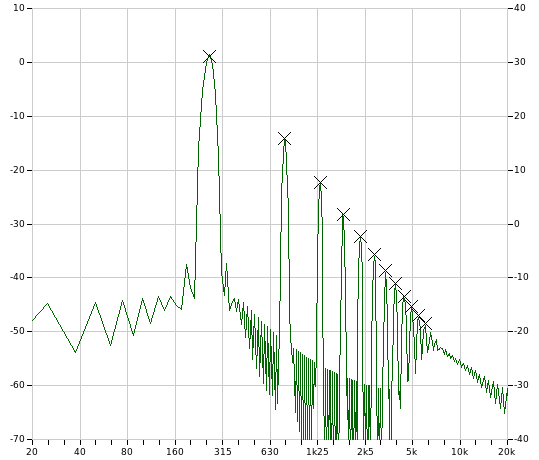
\includegraphics[width=80mm]{analysis/manual_i_compare.png}
\caption{Comparison between emulated and real manual I drawbar 8' sounds.}
% Manual
\label{fig:comp_manual_i}
\end{figure}



\subsection{Section II}

As described earlier in section \ref{section:sections}, Section II has a controllable brightness feature. The variable brightness is done by dividing each bus bar into two streams, one of which is high-passed and the other low-passed. The streams derived from different bus bars are then mixed together into bright and dull streams. The brightness control is a simple balance control between the two streams. 

%The original organ has a slight -3dB dip at the center of the control which is not emulated as it reduces the use of center positions dramatically. The dip 

The high-pass filtering is done by a two stage RC filter with a resistor in parallel with the capacitor of the first filter. Thus the filter is effectively a shelving high pass filter. The shelf is emulated by calculating a voltage divider between the parallel resistor and the resistor in the RC high pass filter. The voltage divider gives a gain coefficient \emph{C} which is used to mix together the high-passed and unfiltered signals. Unfiltered signal is multiplied by \emph{C} while the filtered is multiplied by \emph{1-C} and the results are added together. This keeps gain at high frequencies at 0dB as with the original passive filter. The two passive filters also affect each other and cannot be emulated by simply chaining two digital filters. The load applied by two filter stages is emulated by dividing the resistance of one filter by two. This doubles the cutoff frequency of the filter. This method was found by trial and error. Figure \ref{fig:manual_ii_hp} shows the block diagram of the complete filter.

The low-pass stage is much more straightforward. Filtering consists of two chained RC low-pass filters. However, the best match with the original organ was achieved by not compensating for load posed by the chained filters. Thus the filter stage is just two digital RC low pass filters.

Figure \ref{fig:comp_manual_ii} shows C3 played on a fully bright manual II with only the 8' draw bar engaged. The line depicts the frequency spectrum of the emulation output. The crosses show peaks measured from a YC-20 organ using the same settings. This measurement was done at the same overall level as measurements in figure \ref{fig:comp_manual_i}. This shows that there are some overall volume issues between the two manuals, but the balance between harmonics of the sound is well emulated.

\begin{figure}[tbp]
\centering
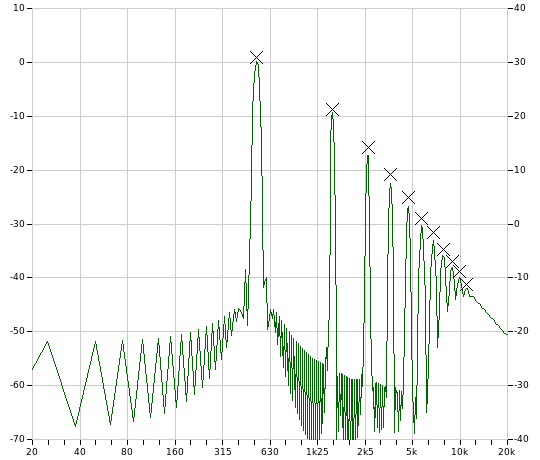
\includegraphics[width=80mm]{analysis/manual_ii_compare.png}
\caption{Comparison between emulated and real bright manual II drawbar 8' sounds.}
\label{fig:comp_manual_ii}
\end{figure}

\subsection{Percussion}

The percussion uses the signal on the 1' bus bar to trigger an envelope generator. There is a root-mean-square envelope follower on the 1' bus bar and the envelope is triggered when the follower exceeds a set threshold. The envelope generator starts off with a signal where a one frame unit impulse is created at the trigger point. This impulse signal is low-pass filtered to match the measured percussion envelope. This envelope is then used to control the volume of a mix of the 1', 2-2/3' and 16' bus bars. Some bleed is added to the envelope generator output to emulate the bleed exhibited by the real organ.

\subsection{Bass manual}

Emulating the bass section perfectly is a complex task due resistor mixing and the variable impedances per drawbar for the RC filter. Measurements from the real organ however suggest that the low frequency fundamentals dominate the signal and an acceptable emulation is achieved by carefully controlling the mix of the bass bus bars and by using a single fixed RC lowpass filter. This one filter is applied to a mix of both bass draw bars.

\section{Performance}
\label{section:performance}

Running this emulation requires a substantial amount of processing power. There are 96 oscillators working all of the time and there are hundreds of filters being applied at many stages of the design. Faust is designed to easily harness multiple processing units in parallel. The design of the emulation has a lot of potential for parallelization and as such, it should work as a good real world test for Faust's SMP features.

The performance numbers shown here are measured using a modified version of the Faust benchmarking suite. These numbers are estimates of achieved memory bandwidth and as such, the results are in megabytes of audio data generated per second. The Faust benchmark uses this measurement, as memory bandwidth on SMP systems is a precious commodity. In the case of the YC-20, the processing creates much more data than what comes out of its single mono output. Thus the figures can only be compared to each other.

Tests were ran on a Dell D820 laptop with a Core 2 Duo T7400 (2.16GHz) processor using the internal sound interface. The operating system was 32 bit Ubuntu 9.10. The processor frequency governor was switched to performance on both cores before running the tests. The kernel was a standard Ubuntu package, 2.6.31-19-generic and the used gcc version was 4.4.1-4ubuntu9. Benchmarks were done on YC-20 code revision 227\footnote{Subversion repository available at http://foo-plugins.googlecode.com/svn/trunk/}. Figures in column C are from a slightly modified version of the YC-20 code and it shows the performance impact of non-branching PolyBLEP calculations. The results in MB/s are shown in table \ref{table:performance}.

\begin{table}[h]
 \begin{center}
\begin{tabular}{|l|l|l|l|}

      \hline
      Faust benchmark          & (A)  & (B)  & (C) \\
      \hline\hline
      scalar (galsascal)       & 0.40 & 0.43 & 0.28 \\
      vectorized (galsavec)    & 0.58 & 0.59 & 0.35 \\
      vectorized 2 (galsavec2) & 0.62 & 0.62 & 0.34 \\
      OpenMP (galsomp2)        & 0.51 & 0.55 & 0.29 \\
      scheduler (galsasch)     & 0.90 & 0.88 & N/A \\
      scheduler 2 (galsasch2)  & 0.93 & 0.89 & N/A \\
      \hline

\end{tabular}
\caption{The tests were ran with different sets of gcc parameters: \\
(A) Branching C++ PolyBLEP evaluations. gcc -O3 -march=native -mfpmath=sse -msse -msse2 -msse3 -ffast-math -ftree-vectorize \\
(B) Branching C++ PolyBLEP evaluations. gcc -O3 -march=native -mfpmath=sse -msse -msse2 -msse3 -ffast-math -ftree-vectorize -fgcse-sm  -funsafe-math-optimizations \\
(C) Divider slave oscillators use non-branched PolyBLEP operations. gcc -O3 -march=native -mfpmath=sse -msse -msse2 -msse3 -ffast-math -ftree-vectorize -fgcse-sm  -funsafe-math-optimizations \\
GCC was unable to compile the scheduler versions of the emulation with non-branching PolyBLEP operations.\\
}\label{table:performance}
 \end{center}
\end{table}

There was notable variance between consecutive test runs, so the only real results deductible from the tests shown in table \ref{table:performance} is that the scheduler mode gives the best performance. This data is backed by tests done by measuring the performance of the YC-20 emulation running as a jack application. The measurements shown in table \ref{table:performance2} were done by running the emulation compiled with different flags and observing the DSP percentage meter in qjackctl. This meter tells how much of the time between jack engine callbacks is spent processing jack client callbacks.

\begin{table}[h]
 \begin{center}
\begin{tabular}{|l|l|l|}

      \hline
      Tests         & Faust flags & Load   \\
      \hline\hline
      scalar        & none & $\sim$ 49\% \\
      vectorized    & -vec -vs 32 & $\sim$ 34\% \\
      scheduler     & -sch -g -vs 256 & $\sim$ 29\% \\
      \hline

\end{tabular}
\caption{All tests were compiled with the following gcc flags: \\
-O3 -march=native -mfpmath=sse -msse -msse2 -msse3 -ffast-math -ftree-vectorize. \\
Jack 1 was running real-time with a dummy back-end simulating a 48kHz sample rate with 512 frame buffers.
}\label{table:performance2}
 \end{center}
\end{table}



\section{Conclusions}

While there is still some way to go for an accurate emulation of the YC-20 organ, this work has created a usable combo-organ synthesizer which sounds very much like the real YC-20. The remaining work is mostly meticulous filter tuning. A better quality anti-aliasing method could be useful although the available methods will come at the expense of even more CPU cycles. The real organ also has considerable bleed and inconsistencies which might be worth emulating.

\subsection{How to improve Faust}

As discussed in section \ref{section:tone-generation}, and shown in the results in section \ref{section:performance}, there is a strong case for a truly branching select operation. However, the semantics of Faust requires all of the processing graph to be evaluated for every frame. Truly branching operations would cause some function evaluations to be skipped. The operating semantics are however compatible with branching operations if the skipped functions are stateless. This is because if the function has no state, the next evaluation of the function does not depend on previous evaluations.

There are two ways truly branching operations can be added to Faust: either select2 and select3 calls with no stateful function branches are compiled automatically as truly branching or a new branching select call is created. Both cases require the specification of rules on what a stateless function is. Also, the compiler must check whether the functions being skipped over comply to these specifications before allowing compilation of such code.

This logic could also be generalized to multiplication functions. Function $f(x)$ in equation \ref{eq:comp-op} is an example of a function where evaluating $t2(x)$ can be skipped if $x \leq 0$ as $t1(x)$ evaluates to 0 for $x \leq 0 $ and $t2$ is stateless.

\begin{equation}
\label{eq:comp-op}
\begin{split}
t1(x) &= (x>0) \\
t2(x) &= x^2-fmod(x,1.0) \\
f(x)  &= t1(x) * t2(x) \\
\end{split}
\end{equation}

%Branchless select2 and select3 can very efficient in some cases, but sometimes true branches are required.

The compiler error messages are often unhelpful. They do not always specify in which file the compilation error occurred. Optimally the compiler should identify the file name, line number and if possible, the name of the function the error occurred in. One specific issue with the compiler messages is worth giving special attention to. It is cases where the number of inputs and outputs of functions in a sequential composition do not match. In such cases Faust outputs a quite exhaustive description of the functions in the composition instead of just the names of the functions. For example, if the YC-20 emulation would fail to cut the phase output of the last divider (dividers would then output 108 instead of 96 streams), the resulting error message is 67 kilobytes.

For signal processing, the lack of support for Fourier transforms restricts what problems can be solved. As mentioned in section \ref{section:tone-generation}, the better band-limiting method (BLEP) is not possible to implement in pure Faust. Fourier transforms would naturally be useful for a variety of other tasks as well. Fortunately there has been promising news of multi-rate support for Faust which would allow processing such as Fourier transforms.

As procedural programming is the prevailing model of programming, it is safe to say many potential users of Faust are familiar with only that model. This applies pressure to the quality of documentation. The current documentation should abbreviate the definitions of the more advanced features of the language. Mainly recursion and the rdtable and rwtable functions could benefit from better explanations. Currently the functions are almost side-stepped and almost nothing but their function syntax is described.

Implementing the matrix mixer required a lot of hand-crafting. Having a concept of indexable arrays would help such operations. If the 96 inputs of the keyboard mixer and the buttons representing the keys of the organ could be arranged into arrays, the mixing could be done algorithmically using the aggregate functions such as sum. Such operations could surely open up possibilities of optimizing the created C++ code. As it stands, the keyboard mixing is compiled into a large amount of separate discrete multiplication and addition operations which can not be vectorized.

The Faust code shown as equation \ref{eq:ambiguous} is ambiguous, but can be compiled without any warning. This can lead to anywhere from unexpected results to complete failure. It would be good form for the Faust compiler to at least warn the user of the situation.

\begin{equation}
\label{eq:ambiguous}
\begin{split}
f(x , y) = x + y\\
with \{ x = y * y; \};\\
\end{split}
\end{equation}


% DSP processors?

%Size of created code: often used functions are rewritten leading to slow compilation and huge amounts of local variables.

\subsection{Benefits of Faust}

Functional thinking suits audio applications very well, as solutions to problems can often be expressed as mathematical equations. This model sidesteps many of the issues procedural programs face, as the processors can be expressed at a higher abstraction level. Unlike with procedural languages, Faust allows programmers to not worry about buffers, their lengths or offsets or loop structures. This also saves time as the programmer can concentrate on processing instead of debugging issues with transferring buffers and interpreting offsets and buffer lengths.

Faust code is easy to keep readable as the syntax offers tools, such as sequential composition, which help keep functions simple and concise. See listings \ref{list:c-consec}, \ref{list:c-enclosed} and \ref{list:faust} for an example. While listing \ref{list:c-enclosed} is pretty compact, one should note that functions are presented to the reader in reverse order and it is also difficult to see to which function return value the multiplication is applied to.

\begin{lstlisting}[language=C,label=list:c-consec,caption=Consecutive calls]
float dostuff(float f) {
	f = func1(f);
	f = func2(f);
	f = f * 2.5;
	f = func3(f);
	return f;
}
\end{lstlisting}

\begin{lstlisting}[language=C,label=list:c-enclosed,caption=Enclosed statements]
float dostuff(float f) {
	return func3( func2( func1(f)) * 2.5 );
}
\end{lstlisting}

\begin{lstlisting}[language=C,label=list:faust,caption=Faust sequential composition]
dostuff = func1 : func2 : *(2.5) : func3;
\end{lstlisting}

The SVG output of the Faust compiler is also worth mentioning. The compiler can create hyper-linked SVG documents which depict the whole process function. This document can be an excellent learning and debugging tool as it shows how the compiler understood the compiled code. Figure \ref{fig:manual_ii_hp} shows an example of this output.

\begin{figure}[tbp]
\centering
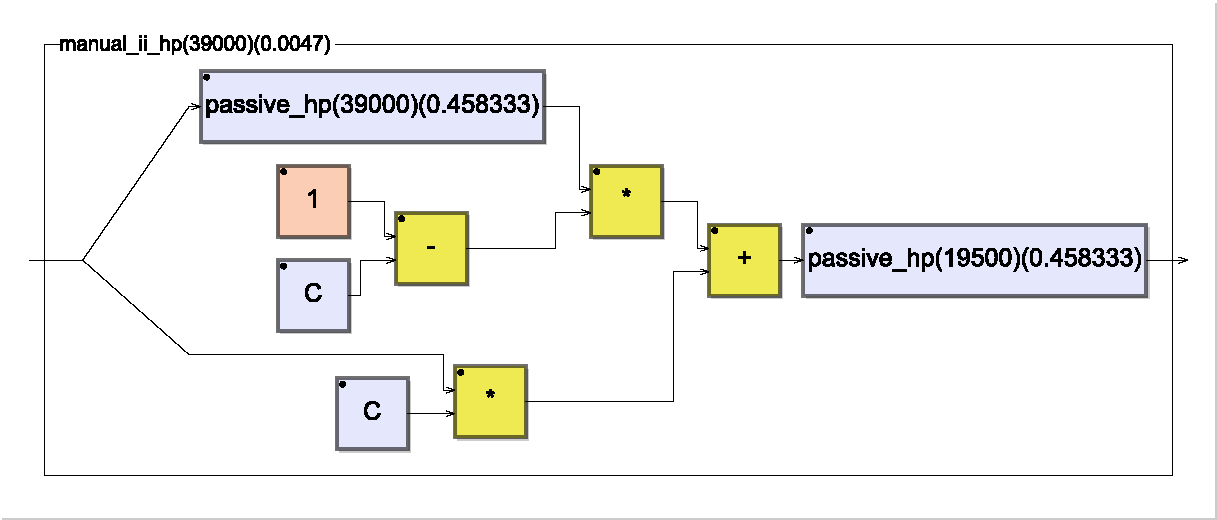
\includegraphics[height=60mm,angle=270]{manual_ii_hp.pdf}
\caption{Faust SVG output of manual II high pass filtering for a single draw bar. The parameters for the filters are resistance in ohms and capacitance in microfarads.}
\label{fig:manual_ii_hp}
\end{figure}

The stream concept also makes code reusable. When combining procedural code from multiple parties you often need to either convert data types between the different modules or refactor the modules to match. Faust processors naturally fit with each other. This model works very well with open source as it make easy to spread good ideas and implementations. It might even lead to a resource library of truly reusable components usable with any Faust project -- as long as the licenses are compatible.

Faust also provides automatic parallelization and vectorization. This allows access to these advanced optimization methods which usually require expert programming skills to implement. These capabilities have been discussed in detail by Orlarey, Fober and Letz\cite{orlarey:09a}. Faust also allows the developer to easily test and compare different optimization methods without refactoring their code.

\section{Acknowledgements}

Thanks to Petri Junno for support and all the help with analyzing the original organ. I would also like to thank Sakari Bergen, Torben Hohn and Yann Orlarey for providing advice.

\bibliographystyle{acl}
\bibliography{lac2010_yc20}

\end{document}
